\documentclass[xcolor={dvipsnames},aspectratio=169,10pt]{beamer}

% utility packages
\usepackage{etoolbox}
\usepackage{multicol}
\usepackage{relsize}

% better text justifying
\usepackage{microtype}
% justify text inside list environment
% Ref: http://liam0205.me/2017/04/11/justifying-in-beamer-s-lists/
\usepackage{ragged2e}
\makeatletter
\patchcmd{\itemize}{\raggedright}{\justifying}{}{}
\patchcmd{\beamer@enum@}{\raggedright}{\justifying}{}{}
\patchcmd{\@@description}{\raggedright}{\justifying}{}{}
\makeatother

% math related packages
\usepackage{amsmath}
\usepackage[ruled,vlined]{algorithm2e}
\SetAlCapNameFnt{\scriptsize}
\SetAlCapFnt{\scriptsize}
\SetAlFnt{\scriptsize}

% figure related packages
\usepackage{graphicx}
\usepackage[scale=2]{ccicons}
\usepackage{qrcode}
\usepackage{tikz}
\usepackage{tikzpagenodes}
\usetikzlibrary{positioning}

% table related packages
\usepackage{array}
\usepackage{booktabs}
\usepackage{multirow}
\usepackage{colortbl}
\newcommand{\tabincell}[2]{\begin{tabular}{@{}#1@{}}#2\end{tabular}}

% code highlight
\usepackage{listings}
\usepackage{minted}
\definecolor{mintedbg}{HTML}{E5E9F0}
\setminted{autogobble,bgcolor=mintedbg,fontsize=\small}
\setmintedinline{bgcolor=mintedbg,fontsize=\smaller}
\newminted{bash}{}
\newminted{latex}{}
\newmintinline{bash}{}
\newmintinline{latex}{}
\newcommand{\texdoc}[2]{\href{#2}{\bashinline|texdoc #1|}}

% hyperref setting
\hypersetup{
  unicode,
  psdextra,
  bookmarksnumbered=true,
  bookmarksopen=true,
  bookmarksopenlevel=3,
  bookmarksdepth=4,
  pdfcenterwindow=true,
  pdfstartview={Fit},
  pdfpagemode={FullScreen},
  pdfpagelayout={SinglePage},
}
\usepackage{bookmark}

% beamer theme
\usetheme{metropolis}
\metroset{block=fill,numbering=fraction}

% caption style
\usepackage{subcaption}
\setlength\abovecaptionskip{3pt}
\setbeamerfont{caption}{size=\scriptsize}
\renewcommand{\figurename}{Fig.}
\captionsetup{labelformat=empty,labelsep=none,textfont={bf,it}}

% Ref: https://github.com/gpoore/minted/blob/master/source/minted.dtx
\newenvironment{latexexample}
{\VerbatimEnvironment\begin{VerbatimOut}[gobble=3]{example.out}}{\end{VerbatimOut}%
  \begin{center}
    \begin{minipage}{0.47\linewidth}%
      \inputminted[resetmargins,fontsize=\scriptsize]{latex}{example.out}%
    \end{minipage}%
    \hspace{0.05\linewidth}%
    \begin{minipage}{0.47\linewidth}%
      \begin{framed}
        \setlength{\parindent}{2em}%
        \input{example.out}%
      \end{framed}
    \end{minipage}%
  \end{center}
}

\newenvironment{mathexample}
{\VerbatimEnvironment\begin{VerbatimOut}[gobble=3]{example.out}}{\end{VerbatimOut}%
  \begin{center}
    \begin{minipage}{0.47\linewidth}%
      \inputminted[resetmargins,fontsize=\scriptsize]{latex}{example.out}%
    \end{minipage}%
    \hspace{0.05\linewidth}%
    \begin{minipage}{0.47\linewidth}%
      \begin{framed}
        \[ \input{example.out} \]
      \end{framed}
    \end{minipage}%
  \end{center}
}

\newenvironment{mathexamples}
{\VerbatimEnvironment\begin{VerbatimOut}[gobble=3]{example.out}}{\end{VerbatimOut}%
  \begin{center}
    \begin{minipage}{0.47\linewidth}%
      \inputminted[resetmargins,fontsize=\scriptsize]{latex}{example.out}%
    \end{minipage}%
    \hspace{0.05\linewidth}%
    \begin{minipage}{0.47\linewidth}%
      \begin{framed}
        \directlua{
          local first = true
          for line in io.lines('example.out') do
          if first then
          first = false
          else
          tex.print('\\newline ')
          end
          tex.print('$' .. line .. '$')
          end
        }
      \end{framed}
    \end{minipage}%
  \end{center}
}


\title{Introduction to \LaTeX}
\subtitle{Writing papers the right way}
\author{Cheng XU}
\date{September 26, 2019}
\titlegraphic{
  \begin{tikzpicture}[overlay, remember picture]
    \node[%
      above right=0.35cm and -0.2cm of current page footer area.south west,
      anchor=south west,
      inner sep=0pt] {%
      \usebeamerfont{footline}
      \begin{tabular}{lm{.8\textwidth}}
        \href{http://creativecommons.org/licenses/by/4.0/}{\ccby} &
        This work is licensed under a \href{http://creativecommons.org/licenses/by/4.0/}{Creative Commons ``Attribution 4.0 International''} license. \par
        Get source of this slides and example document from \url{https://github.com/xu-cheng/latex-tutorial}.
      \end{tabular}
    };
    \node[%
      above left=0.35cm and 0cm of current page footer area.south east,
      anchor=south east,
      inner sep=0pt]{\qrcode[height=1.5cm]{https://github.com/xu-cheng/latex-tutorial}};
  \end{tikzpicture}
}

\begin{document}

\maketitle%

\begin{frame}{Contents}
  \setbeamertemplate{section in toc}[sections numbered]
  \tableofcontents[hideallsubsections]
\end{frame}

\section{Getting Started with \LaTeX}

\begin{frame}{Introduction}
  \begin{itemize}
    \item \alert{\LaTeX{}} is a document preparation system and document markup language.
    \item It can be used to typeset articles, books, slides, posters, even graphics.
    \item \textbf{\textcolor{Green}{Pros}:}
          \begin{itemize}
            \item It separates presentation/format from contents.
            \item Since the source codes are plaintext, it works well with version control system such as git.
            \item Highly customizable through various of packages.
          \end{itemize}
    \item \textbf{\textcolor{Red}{Cons}:}
          \begin{itemize}
            \item There is no graphic interface to support WYSIWYG style editing.
            \item Not suitable to produce unstructured documents.
          \end{itemize}
  \end{itemize}
\end{frame}

\begin{frame}[fragile]{Installation}
  \begin{itemize}
    \item \textbf{Windows/Linux}
          \begin{itemize}
            \item TeXLive \url{https://www.tug.org/texlive/}
            \item Online installer:
                  \begin{itemize}
                    \item Windows \\ \url{http://mirror.ctan.org/systems/texlive/tlnet/install-tl-windows.exe}
                    \item Linux \\ \url{http://mirror.ctan.org/systems/texlive/tlnet/install-tl-unx.tar.gz}
                  \end{itemize}
            \item Offline ISO file:
                  \footnotesize
                  \url{http://mirror.ctan.org/systems/texlive/Images/}
          \end{itemize}
    \item \textbf{Mac}
          \begin{itemize}
            \item MacTeX \url{http://www.tug.org/mactex/}
            \item Or install through Homebrew (\url{https://brew.sh}) \\
                  \begin{minipage}{\linewidth+2.1em}
                    \inputminted[fontsize=\scriptsize]{bash}{./minted/install_mactex.sh}
                    \vspace{-2ex}
                  \end{minipage}
          \end{itemize}
    \item TeXLive/MacTeX release major updates around May each year. \\
          It is recommended to uninstall the old version and install the new version annually.
  \end{itemize}
\end{frame}

\begin{frame}{\LaTeX~editor}
  \begin{itemize}
    \item \LaTeX~source codes are plaintext. So you can use any editor you like.
    \item \textbf{Visual Studio Code \alert{[Recommend]}}
          \begin{itemize}
            \item \footnotesize \url{https://code.visualstudio.com}
            \item LaTeX Workshop \footnotesize \url{https://github.com/James-Yu/LaTeX-Workshop}
            \item Code Spell Checker \footnotesize \url{https://github.com/streetsidesoftware/vscode-spell-checker}
          \end{itemize}
    \item \textbf{Vim/Neovim}
          \begin{itemize}
            \item \footnotesize \url{https://www.vim.org} | \url{https://neovim.io}
            \item Vimtex \footnotesize \url{https://github.com/lervag/vimtex}
          \end{itemize}
    \item \textbf{Emacs}
          \begin{itemize}
            \item \footnotesize \url{https://www.gnu.org/s/emacs}
            \item AUCTeX \footnotesize \url{https://www.gnu.org/software/auctex}
          \end{itemize}
    \item \textbf{TeXstudio}
          \begin{itemize}
            \item \footnotesize \url{https://www.texstudio.org}
          \end{itemize}
  \end{itemize}
\end{frame}

\begin{frame}{Overleaf}
  \begin{itemize}
    \item \alert{Overleaf} (\url{https://www.overleaf.com/}) is a online, collaborative LaTeX editor
    \item Free for personal use
    \item \$15/month to share project among up to 10 collaborators
  \end{itemize}

  \begin{figure}
    \centering
    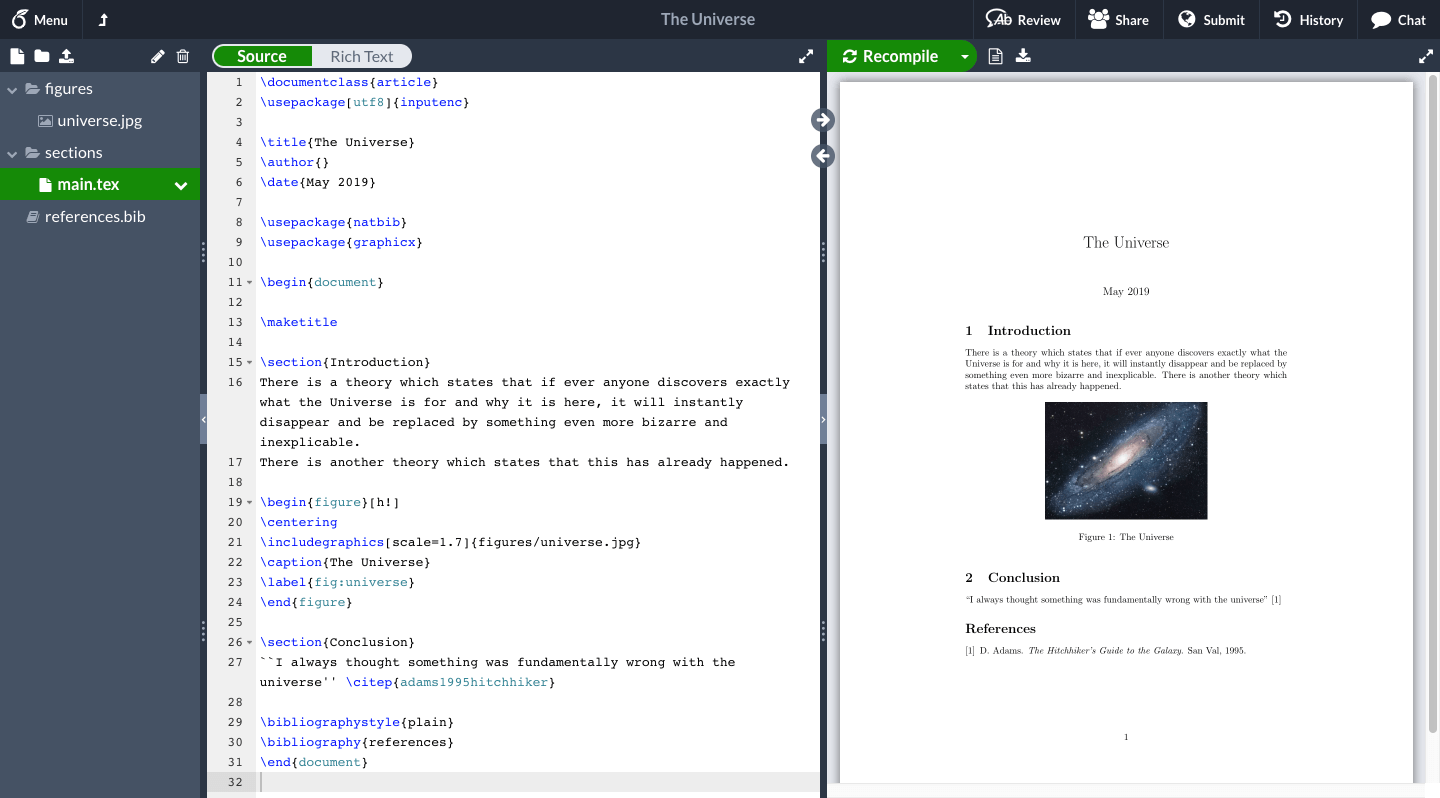
\includegraphics[width=.7\linewidth]{./figs/overleaf.png}
  \end{figure}
\end{frame}

\section{A Basic Document}

\begin{frame}[fragile]{Hello, \LaTeX!}
  \begin{columns}
    \begin{column}{.7\linewidth}
      \begin{itemize}
        \item Create \mintinline{text}|hello.tex| file with following content.
              \inputminted{latex}{./minted/hello.tex}
        \item Compile it
              \begin{itemize}
                \item Click the build button in your \LaTeX~editor/IDE
                \item OR using command line: \bashinline|latexmk -pdf hello|
              \end{itemize}
        \item Open \mintinline{text}|hello.pdf| to preview the result
      \end{itemize}
    \end{column}
    \begin{column}{.3\linewidth}
      \begin{figure}
        \centering
        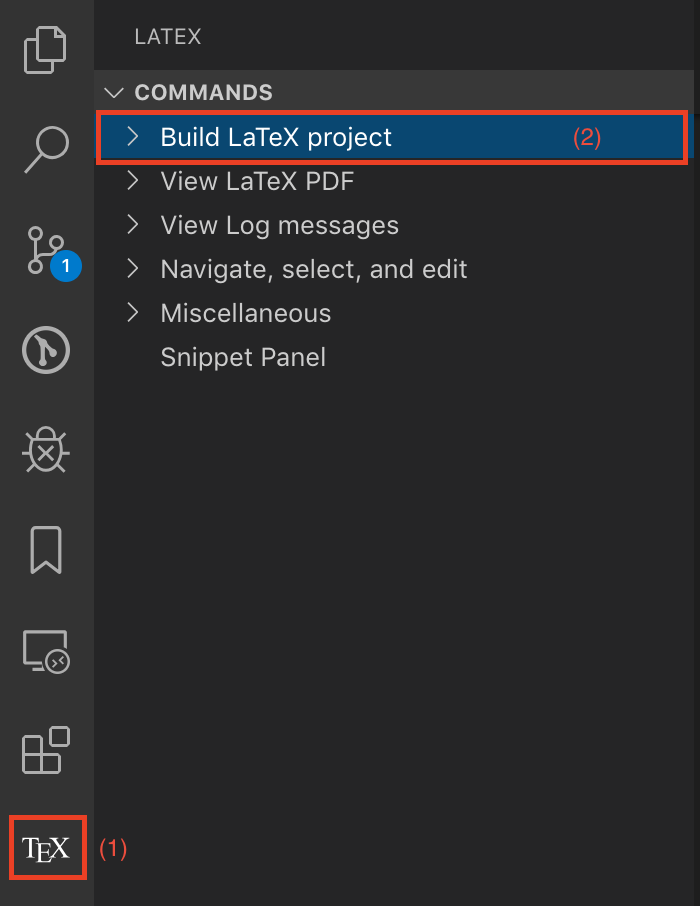
\includegraphics[width=\linewidth]{./figs/vscode-compile-project.png}
        \caption{Compile \LaTeX~Project in VSCode}
      \end{figure}
    \end{column}
  \end{columns}
\end{frame}

\begin{frame}[fragile]{Example of A Complex Document}
  \begin{itemize}
    \item Download the source code from \url{https://github.com/xu-cheng/latex-tutorial/archive/master.zip}
    \item The example document is located in the \mintinline{text}|example| folder. It contains:
          \begin{itemize}
            \item \mintinline{text}|main.tex| The main tex source
            \item \mintinline{text}|preamble.tex| A subfile to store format definitions
            \item \mintinline{text}|tikz-example.tex| A figure drawn using tikz
            \item \mintinline{text}|ref.bib| A database of references
          \end{itemize}
    \item Use \bashinline|latexmk -pdf main| to compile the document
    \item Access the same example in Overleaf: \url{https://www.overleaf.com/read/qsthqbjphhrz}
  \end{itemize}
\end{frame}

% \begin{noindent}
\begin{frame}[fragile]{Comment, Command and Environment}
  \begin{itemize}
    \item \latexinline|%| starts a comment. e.g.~\latexinline|% this is hello.tex|
    \item \latexinline|\| starts a command.
          \begin{latexcode}
            \command % a command
            \command{} % also a command
            \command{arg} % a command with an argument
            \command{arg1}{arg2} % a command with multiple arguments
            \command[opt arg]{arg} % [] is for optional argument
          \end{latexcode}
    \item \latexinline|\begin{} ... \end{}| denotes an environment
          \begin{latexcode}
            \begin{envname}
              inside the environment
            \end{envname}
            % LaTeX environment can take arguments
            \begin{envname}{arg} \end{envname}
            \begin{envname}[opt arg]{arg} \end{envname}
          \end{latexcode}
  \end{itemize}
\end{frame}
% \end{noindent}

\begin{frame}[fragile]{Source File Structure}
  \begin{itemize}
    \item A document starts with \latexinline|\documentclass{...}| command to specify the template
    \item Common templates include:
          \setlength{\multicolsep}{0pt}
          \setlength{\columnsep}{0pt}
          \begin{multicols}{3}
            \begin{itemize}
              \item \texttt{article}
              \item \texttt{book}
              \item \texttt{report}
              \item \texttt{letter}
              \item \texttt{beamer} \textsmaller{(slides)}
              \item \texttt{standalone} \textsmaller{(graphics)}
              \item \texttt{acmart} \textsmaller{(ACM~template)}
              \item \texttt{IEEEtrans} \textsmaller{(IEEE~template)}
              \item[]
            \end{itemize}
          \end{multicols}
    \item Template class can accept options, e.g.~\latexinline|\documentclass[a4paper,10pt]{article}|
  \end{itemize}

  \begin{block}{Class Options for \texttt{article}, \texttt{report}, \texttt{book}, \texttt{letter}}
    \begin{description}[\scriptsize\texttt{titlepage}, \texttt{notitlepage}]
      \scriptsize
      \item[\normalfont\texttt{10pt}, \texttt{11pt}, \texttt{12pt}] \quad Set font size.
      \item[\normalfont\texttt{a4paper}, \texttt{letterpaper}, \ldots] \quad Defines
            the paper size.
      \item[\normalfont\texttt{fleqn}] \quad Typesets displayed formulae left-aligned
            instead of centred.
      \item[\normalfont\texttt{leqno}] \quad Places the numbering of formulae on the
            left hand side instead of the right.
      \item[\normalfont\texttt{titlepage}, \texttt{notitlepage}] \quad Specifies whether a new page should be started after the document title or not.
      \item[\normalfont\texttt{onecolumn}, \texttt{twocolumn}] \quad Typeset the document in one column or two columns.
      \item[\normalfont\texttt{twoside, oneside}] \quad Specifies whether double or single sided output should be generated.
      \item[\normalfont\texttt{landscape}] \quad Changes the layout of the document to print in landscape mode.
      \item[\normalfont\texttt{openright, openany}] \quad Makes chapters begin either only on right hand pages or on the next page available.
    \end{description}
  \end{block}
\end{frame}

% \begin{noindent}
\begin{frame}[fragile]{Source File Structure}
  \begin{itemize}
    \item The region after \latexinline|\documentclass| and before \latexinline|\begin{document}| is called \alert{preamble}.
    \item You can load packages and define format of the document here, e.g.~\latexinline|\usepackage{amsmath}|
    \item Package can be loaded with options, e.g.~\latexinline|\usepackage[style=ieee]{biblatex}|
    \item To find the package document:
          \begin{itemize}
            \item Run \bashinline|texdoc <pkg_name>| in command line
            \item \url{http://www.texdoc.net}
          \end{itemize}
    \item You start the body of the text with \latexinline|\begin{document}|.
    \item Finally, \latexinline|\end{document}| denotes the end of the document.
  \end{itemize}
\end{frame}
% \end{noindent}

\section{Typesetting Text}

\begin{frame}[fragile]{Syntax}
  \begin{itemize}
    \item The main body of \LaTeX{} code is plain text.
    \item \LaTeX{} treats contiguous spaces or a single linebreak as a single space. \\
          It starts a new paragraph after empty lines.
          \begin{latexexample}
            It does not matter whether
            you enter one or several
            spaces        after a word.

            An empty line starts a new
            paragraph.
          \end{latexexample}
    \item \latexinline|\\| or \latexinline|\newline| starts a new line without starting a new paragraph.
  \end{itemize}
\end{frame}

\begin{frame}[fragile]{Special Characters and Symbols}
  \begin{itemize}
    \item Certain characters are reserved, you need to use escape command to typeset them.
          \begin{latexexample}
            \# \$ \% \^{} \& \_ \{ \} \~{}
            \textbackslash
          \end{latexexample}
    \item \latexinline|`text'| and \latexinline|``text''| typeset `single quoted text' and ``double quoted text''
    \item There are four kinds of dashes
          \begin{itemize}
            \item \textbf{hyphen}: \latexinline|-|, e.g.~part-time
            \item \textbf{en-dash}: \latexinline|--|, e.g.~Pages 1--10
            \item \textbf{em-dash}: \latexinline|---|, e.g.~yes---or no?
            \item \textbf{minus sign}: \latexinline|-| inside math environment, e.g.~$-1$
          \end{itemize}
    \item Use \latexinline|\ldots| instead of \latexinline|...| to typeset ellipsis, e.g.~a, b, c, \ldots
  \end{itemize}
\end{frame}

\begin{frame}[fragile]{Font Face \& Size}
  \begin{table}
    \centering
    \begin{tabular}{@{}>{\columncolor{mintedbg}}ll@{\qquad}>{\columncolor{mintedbg}}ll@{}}
      \latexinline|\textrm{...}|     & \textrm{roman}             &
      \latexinline|\textsf{...}|     & \textsf{sans serif}          \\
      \latexinline|\texttt{...}|     & \texttt{typewriter}        &
                                     &                              \\
      \latexinline|\textmd{...}|     & \textmd{medium}            &
      \latexinline|\textbf{...}|     & \textbf{bold face}           \\
      \latexinline|\textup{...}|     & \textup{upright}           &
      \latexinline|\textit{...}|     & \textit{italic}              \\
      \latexinline|\textsl{...}|     & \textsl{slanted}           &
      \latexinline|\textsc{...}|     & \textsc{small caps}          \\
      \latexinline|\emph{...}|       & \emph{emphasized}          &
      \latexinline|\textnormal{...}| & \textnormal{document font}
    \end{tabular}
    \caption{Font Face Commands}
  \end{table}

  \begin{itemize}
    \item Put the text inside the above commands to change the font face. \\
          e.g.~\latexinline|\textbf{this text will be in bold face}|
  \end{itemize}
\end{frame}

\begin{frame}[fragile]{Font Face \& Size}
  \begin{columns}
    \begin{column}{0.5\textwidth}
      \begin{table}
        \centering
        \begin{tabular}{@{}>{\columncolor{mintedbg}}ll}
          \latexinline|\tiny|         & {\tiny tiny font}                \\
          \latexinline|\scriptsize|   & {\scriptsize very small font}    \\
          \latexinline|\footnotesize| & {\footnotesize quite small font} \\
          \latexinline|\small|        & {\small small font}              \\
          \latexinline|\normalsize|   & {\normalsize normal font}        \\
          \latexinline|\large|        & {\large large font}              \\
          \latexinline|\Large|        & {\Large large font}              \\
          \latexinline|\LARGE|        & {\LARGE very large font}         \\
          \latexinline|\huge|         & {\huge huge}                     \\
          \latexinline|\Huge|         & {\Huge largest}
        \end{tabular}
        \caption{Font Size Commands}
      \end{table}
    \end{column}
    \begin{column}{0.5\textwidth}
      \begin{itemize}
        \item These commands will affect font size in the following text
        \item Use \latexinline|{ ... }| to limit its effect range   \\
              e.g.~\latexinline|{\small small size text}|
      \end{itemize}
    \end{column}
  \end{columns}

\end{frame}

\begin{frame}[fragile]{Spacing}
  \begin{itemize}
    \item Use package \href{http://texdoc.net/texmf-dist/doc/latex/geometry/geometry.pdf}{\emph{geometry}} to change the paper margin
          \begin{latexcode}
            \usepackage[top=3cm,bottom=3cm,left=2.5cm,right=2.5cm]{geometry}
          \end{latexcode}
    \item To force a new page, use:
          \begin{itemize}
            \item \latexinline|\newpage|: create a new page
            \item \latexinline|\clearpage|: create a new page and flush all the floats
            \item \latexinline|\cleardoublepage|: In addition to \latexinline|\clearpage|, it makes the next page a right-hand page for two-sided printing
          \end{itemize}
    \item Force a space using \latexinline|~| (unbreakable) or \latexinline|\ | (breakable)
    \item Insert horizontal/vertical spaces with \latexinline|\hspace{1em}| or \latexinline|\vspace{1ex}|
    \item Create a line break and insert vertical spaces using \latexinline|\\ [1ex]|
    \item Fill space using \latexinline|\hfill| or \latexinline|\vfill|
  \end{itemize}
\end{frame}

\begin{frame}[fragile]{Length Unit in \LaTeX}
  \begin{table}
    \centering
    \begin{tabular}{lp{.7\linewidth}}
      \toprule
      \textbf{unit} & \textbf{meaning}                                             \\
      \midrule
      pt            & a point is approximately 1/72.27 inch                        \\
      mm            & a millimeter                                                 \\
      cm            & a centimeter                                                 \\
      in            & inch                                                         \\
      ex            & roughly the height of an `x' (lowercase) in the current font \\
      em            & roughly the width of an `M' (uppercase) in the current font  \\
      mu            & math unit equal to 1/18 em                                   \\
      \bottomrule
    \end{tabular}
    \caption{Length Unit in \LaTeX}
  \end{table}
\end{frame}

\begin{frame}[fragile]{Alignment}
  \begin{latexexample}
    \begin{center}
      text to be centered
    \end{center}

    \begin{flushleft}
      text to be flushed left
    \end{flushleft}

    \begin{flushright}
      text to be flushed right
    \end{flushright}
  \end{latexexample}
\end{frame}

\begin{frame}[fragile]{Hyphenation}
  \begin{itemize}
    \item \LaTeX{} hyphenates words whenever necessary
    \item You can custom the hyphenation using \latexinline|\hyphenation{<word list>}| in the preamble
    \item For example, \latexinline|\hyphenation{FORTRAN Hy-phen-a-tion}| instructs:
          \begin{itemize}
            \item Prevents ``FORTRAN'', ``Fortran'' and ``fortran'' from being hyphenated
            \item Allow ``hyphenation'' to be hyphenated as well as ``Hyphenation''
          \end{itemize}
    \item Or use \latexinline|\-| inserts a discretionary hyphen into a word
          \begin{latexexample}
            I think this is: su\-per\-cal\-%
            i\-frag\-i\-lis\-tic\-ex\-pi\-%
            al\-i\-do\-cious
          \end{latexexample}
    \item \latexinline|\mbox{...}| causes its argument to be kept together under all circumstances
          \begin{latexexample}
            My phone number will change soon.
            It will be \mbox{0116 291 2319}.
          \end{latexexample}
  \end{itemize}
\end{frame}

\begin{frame}[fragile]{Document Structure}
  \begin{itemize}
    \item \LaTeX~is built off the idea \emph{structure} over \emph{formatting}
    \item You can structure the documents using following commands
          \begin{latexcode}
            \part{part name} % only available in book
            \chapter{chapter name} % available in book and report
            \section{section name}
            \subsection{subsection name}
            \subsubsection{subsubsection name}
          \end{latexcode}
    \item The star version commands (e.g.~\latexinline|\section*{}|) suppress the numbering and are not added in the table of contents.
    \item \latexinline|\tableofcontents| can be used to create table of contents.
    \item Use \latexinline|\appendix| to put rest of content in the appendix.
    \item For large project, you can put each chapter/section in a separated file. \\
          Then use \latexinline|\input{file_name}| to include them in the root file.
  \end{itemize}
\end{frame}

\begin{frame}[fragile]{List Structures}
  \begin{itemize}
    \item There are three list structures in \LaTeX
          \begin{latexexample}
            \begin{enumerate}
              \item Item 1
              \item Item 2
            \end{enumerate}
            \begin{itemize}
              \item Item 1
              \item Item 2
            \end{itemize}
            \begin{description}
              \item[key1] Item 1
              \item[key2] Item 2
            \end{description}
          \end{latexexample}
  \end{itemize}
\end{frame}

\begin{frame}[fragile]{List Structures}
  \begin{itemize}
    \item You can use them in nested fashion
          \begin{latexexample}
            \begin{enumerate}
              \item Level 1
                    \begin{enumerate}
                      \item Level 2
                    \end{enumerate}
              \item Level 1
                    \begin{itemize}
                      \item Level 2
                    \end{itemize}
            \end{enumerate}
          \end{latexexample}
  \end{itemize}
\end{frame}

\begin{frame}[fragile]{List Structures}
  \begin{itemize}
    \item Use package \href{http://texdoc.net/texmf-dist/doc/latex/enumitem/enumitem.pdf}{\emph{enumitem}} to custom the list format
          \begin{latexcode}
            \usepackage{enumitem}
            \setlist{noitemsep,partopsep=0pt,topsep=.8ex}
            \setlist[enumerate,1]{label=\arabic*.,ref=\arabic*}
            \newlist{inlineenum}{enumerate*}{1}
            \setlist[inlineenum]{label=(\roman*),ref=(\roman*)}

            \begin{itemize}[label=-]
              \item Item
            \end{itemize}
          \end{latexcode}
  \end{itemize}
\end{frame}

\begin{frame}[fragile]{Math}
  \begin{itemize}
    \item Common mathematical packages
          \begin{latexcode}
            \usepackage{amsmath}
            \usepackage{amssymb}
            \usepackage{amsfonts}
            \usepackage{mathrsfs}
            \usepackage{latexsym}
          \end{latexcode}
    \item List of mathematical symbols \url{https://www.caam.rice.edu/~heinken/latex/symbols.pdf}
    \item ``Short Math Guide for \LaTeX'' (access by \texdoc{short-math-guide}{http://texdoc.net/texmf-dist/doc/latex/short-math-guide/short-math-guide.pdf}) for comprehensive guide
  \end{itemize}
\end{frame}

\begin{frame}[fragile]{Math Mode \& Environment}
  \begin{itemize}
    \item There are two math mode
          \begin{itemize}
            \item  Inline math mode: \latexinline|$\sum_k^n k$| or \latexinline|\(\sum_k^n k\)| to typeset \(\sum_k^n k\)
            \item Display math mode: \latexinline|$$\sum_k^n k$$| or \latexinline|\[\sum_k^n k\]| to typeset
                  \[\sum_k^n k\]
          \end{itemize}
    \item Use \latexinline|equation| environment to number the equation in display mode
          \begin{latexexample}
            \begin{equation}
              E = mc^2
            \end{equation}
          \end{latexexample}
    \item Use \latexinline|\tag| to change the equation label
          \begin{latexexample}
            \begin{equation}
              1 + 1 = 3 \tag{dumb}
            \end{equation}
          \end{latexexample}
  \end{itemize}
\end{frame}

\begin{frame}[fragile]{Math Mode \& Environment}
  \begin{itemize}
    \item Use \latexinline|align| environment to align multiple equations
          % \begin{noindent}
          \begin{latexexample}
            \begin{align}
              B' &=-\nabla \times E, \\
              E' &=\nabla \times B - 4\pi j,
            \end{align}
          \end{latexexample}
          % \end{noindent}
    \item Use \latexinline|\nonumber| to disable the number for some lines
          % \begin{noindent}
          \begin{latexexample}
            \begin{align}
              a &= b + c \nonumber \\
                &= d + e
            \end{align}
          \end{latexexample}
          % \end{noindent}
  \end{itemize}
\end{frame}

\begin{frame}[fragile]{Math Mode \& Environment}
  \begin{itemize}
    \item \latexinline|align*| environment disable the number entirely
          % \begin{noindent}
          \begin{latexexample}
            \begin{align*}
              B' &=-\nabla \times E, \\
              E' &=\nabla \times B - 4\pi j,
            \end{align*}
          \end{latexexample}
          % \end{noindent}
    \item \latexinline|gather|/\latexinline|gather*| display a set of consecutive equations, centered and with no alignment
          % \begin{noindent}
          \begin{latexexample}
            \begin{gather*}
              2x - 5y =  8 \\
              3x^2 + 9y =  3a + c
            \end{gather*}
          \end{latexexample}
          % \end{noindent}
  \end{itemize}
\end{frame}

\begin{frame}[fragile]{Math Symbols}
  \begin{itemize}
    \item The following symbols that can be used directly in math environment
          \begin{mathexamples}
            + - = ! / ( ) [ ] < > | ' : *
          \end{mathexamples}
    \item Greek letters
          \begin{mathexamples}
            \alpha, \beta, \gamma, \pi, \phi, \varphi
          \end{mathexamples}
    \item Operators
          \begin{mathexamples}
            \cos(2\theta) = \cos^2\theta-\sin^2\theta
            \lim\limits_{x \to \infty} \exp(-x) = 0
            a \bmod b
            x \equiv a \pmod{b}
            \log{(N)}
          \end{mathexamples}
  \end{itemize}
\end{frame}

\begin{frame}[fragile]{Math --- Custom Operators}
  \begin{itemize}
    \item You can define your own operators
          \begin{mathexample}
            \operatorname{arg\,max}_a f(a) =
            \operatorname*{arg\,max}_b f(b)
          \end{mathexample}
    \item If it is frequently used,
          \begin{latexcode*}{fontsize=\scriptsize}
            % declared in preamble
            \DeclareMathOperator*{\argmax}{arg\,max} % or \DeclareMathOperator{\argmax}{arg\,max}

            % then used in the document
            \[ \argmax_c f(c) \]
          \end{latexcode*}
  \end{itemize}
\end{frame}

\begin{frame}[fragile]{Math --- Power, Indices, Fraction, Root}
  \begin{itemize}
    \item Powers and indices are equivalent to superscripts and subscripts in normal text mode. The caret (\latexinline|^|) character is used to raise something, and the underscore (\latexinline|_|) is for lowering. If more than one expression is raised or lowered, they should be grouped using curly braces (\latexinline|{| and \latexinline|}|).
          \begin{mathexamples}
            k_{n+1} = n^2 + k_n^2 - k_{n-1}
            n^{22}
            f(n) = n^5 + 4n^2 + 2 |_{n=17}
            \sum_{i=1}^{n} i
            \lim_{x \to \infty} \frac{1}{x}
          \end{mathexamples}
    \item Fraction and root
          \begin{mathexamples}
            \frac{n!}{k!(n-k)!} = \binom{n}{k}
            \sqrt{2}
            \sqrt[n]{1+x+x^2+x^3+\dots+x^n}
          \end{mathexamples}
  \end{itemize}
\end{frame}

\begin{frame}[fragile]{Math --- Delimiters}
  \begin{itemize}
    \item Brackets, braces and delimiters
          \begin{mathexamples}
            ( a ), [ b ], \{ c \}, | d |, \| e \|,
            \langle f \rangle, \lfloor g \rfloor,
            \lceil h \rceil, \ulcorner i \urcorner
          \end{mathexamples}
    \item Automatic sizing
          \begin{mathexamples}
            \left(\frac{x^2}{y^3}\right)
            P\left(A=2\middle|\frac{A^2}{B}>4\right)
            \left\{\frac{x^2}{y^3}\right\}
          \end{mathexamples}
    \item Manual sizing
          \begin{mathexamples}
            ( \big( \Big( \bigg( \Bigg(
          \end{mathexamples}
  \end{itemize}
\end{frame}

\begin{frame}[fragile]{Math --- Matrix}
  \begin{itemize}
    \item Matrices
          \begin{mathexample}
            \begin{matrix}
              a & b & c \\
              d & e & f \\
              g & h & i
            \end{matrix}
          \end{mathexample}
          \begin{mathexample}
            \begin{pmatrix}
              a & b & c \\
              d & e & f \\
              g & h & i
            \end{pmatrix}
          \end{mathexample}
    \item Other matrix environment with different delimiter: \latexinline|bmatrix|, \latexinline|Bmatrix|, \latexinline|vmatrix|, and \latexinline|Vmatrix|
  \end{itemize}
\end{frame}

\begin{frame}[fragile]{Math --- Array}
  \begin{itemize}
    \item Array
          \begin{mathexample}
            \begin{array}{c|c}
              1 & 2 \\
              \hline
              3 & 4
            \end{array}
          \end{mathexample}
          \begin{mathexample}
            f(x) = \left\{
            \begin{array}{ll}
              x & \text{if } x > 0, \\
              0 & \text{otherwise}.
            \end{array}\right.
          \end{mathexample}
    \item Cases
          \begin{mathexample}
            f(x) = \begin{cases}
              x & \text{if } x > 0, \\
              0 & \text{otherwise}.
            \end{cases}
          \end{mathexample}
  \end{itemize}
\end{frame}

\begin{frame}[fragile]{Math Fonts}
  \begin{table}
    \begin{tabular}{>{\columncolor{mintedbg}}ll}
      \latexinline|\mathnormal{...}| & $\mathnormal{ABCDEF~abcdef~123456}$ \\
      \latexinline|\mathrm{...}|     & $\mathrm{ABCDEF~abcdef~123456}$     \\
      \latexinline|\mathit{...}|     & $\mathit{ABCDEF~abcdef~123456}$     \\
      \latexinline|\mathbf{...}|     & $\mathbf{ABCDEF~abcdef~123456}$     \\
      \latexinline|\mathsf{...}|     & $\mathsf{ABCDEF~abcdef~123456}$     \\
      \latexinline|\mathtt{...}|     & $\mathtt{ABCDEF~abcdef~123456}$     \\
      \latexinline|\mathfrak{...}|   & $\mathfrak{ABCDEF~abcdef~123456}$   \\
      \latexinline|\mathcal{...}|    & $\mathcal{ABCDEF}$                  \\
      \latexinline|\mathbb{...}|     & $\mathbb{ABCDEF}$
    \end{tabular}
    \caption{Math Fonts}
  \end{table}
\end{frame}

\begin{frame}[fragile]{Math Spacing}
  \begin{table}
    \centering
    \begin{tabular}{lp{.7\linewidth}}
      \toprule
      \textbf{\LaTeX~code} & \textbf{Description}                                      \\
      \midrule
      \latexinline|\qquad| & twice of \latexinline|\quad| (= 36 mu)                    \\
      \latexinline|\quad|  & space equal to the current font size (= 18 mu)            \\
      \latexinline|\,|     & 3/18 of \latexinline|\quad| (= 3 mu)                      \\
      \latexinline|\:|     & 4/18 of \latexinline|\quad| (= 4 mu)                      \\
      \latexinline|\;|     & 5/18 of \latexinline|\quad| (= 5 mu)                      \\
      \latexinline|\!|     & -3/18 of \latexinline|\quad| (= -3 mu)                    \\
      \latexinline|\ |     & space after backslash, equivalent of space in normal text \\
      \bottomrule
    \end{tabular}
    \caption{Spacing in Math}
  \end{table}
\end{frame}

\begin{frame}[fragile]{Math --- Dots}
  \begin{table}
    \centering
    \begin{tabular}{ll>{\small}p{.7\linewidth}}
      \toprule
      \textbf{\LaTeX~code}       & \textbf{Output} & \textbf{Description}                                                                                                   \\
      \midrule
      \latexinline|\dots|        & $\dots$         & generic dots. It automatically manages whitespaces according to the context, it's a higher level command.              \\
      \latexinline|\ldots|       & $\ldots$        & the output is similar to the previous one, but there is no automatic whitespace management; it works at a lower level. \\
      \latexinline|\cdots|       & $\cdots$        & These dots are centered relative to the height of a letter.                                                            \\
      \latexinline|\vdots|       & $\vdots$        & vertical dots                                                                                                          \\
      \latexinline|\ddots|       & $\ddots$        & diagonal dots                                                                                                          \\
      \latexinline|\hdotsfor{n}| &                 & to be used in matrices, it creates a row of dots spanning $n$ columns.                                                 \\
      \bottomrule
    \end{tabular}
    \caption{Dots in Math}
  \end{table}
\end{frame}

\begin{frame}[fragile]{Math --- Dots}
  \begin{table}
    \centering
    \begin{tabular}{ll>{\small}p{.5\linewidth}}
      \toprule
      \textbf{\LaTeX~code}          & \textbf{Output}   & \textbf{Description}                         \\
      \midrule
      \latexinline|A_1,A_2,\dotsc,| & $A_1,A_2,\dotsc,$ & for ``dots with commas''                     \\
      \latexinline|A_1+\dotsb+A_N|  & $A_1+\dotsb+A_N$  & for ``dots with binary operators/relations'' \\
      \latexinline|A_1 \dotsm A_N|  & $A_1 \dotsm A_N$  & for ``multiplication dots''                  \\
      \latexinline|\int_a^b \dotsi| & $\int_a^b \dotsi$ & for ``dots with integrals''                  \\
      \latexinline|A_1\dotso A_N|   & $A_1\dotso A_N$   & for ``other dots'' (none of the above)       \\
      \bottomrule
    \end{tabular}
    \caption{Semantic Dots in Math}
  \end{table}

  \begin{itemize}
    \item It is recommended to use these semantically oriented commands.
  \end{itemize}
\end{frame}

\begin{frame}[fragile]{Figure and Table}
  \begin{itemize}
    \item To create a float block to place figure or table
          \begin{latexcode}
            % for figure
            \begin{figure} ... \end{figure}
            % for table
            \begin{table} ... \end{table}
            % star version put it across multiple columns
            \begin{figure*} ... \end{figure*}
            \begin{table*} ... \end{table*}
          \end{latexcode}
    \item Positioning can be denoted as an optional argument
          \begin{latexcode}
            \begin{figure}[placement specifier] ... \end{figure}
          \end{latexcode}
  \end{itemize}
\end{frame}

\begin{frame}[fragile]{Figure and Table}
  \begin{table}
    \small
    \begin{tabular}{lp{.8\linewidth}}
      \toprule
      \textbf{Specifier} & \textbf{Description}                                                                                                        \\
      \midrule
      h                  & Place the float here, i.e., approximately at the same point it occurs in the source text (however, not exactly at the spot) \\
      t                  & Position at the top of the page.                                                                                            \\
      b                  & Position at the bottom of the page.                                                                                         \\
      p                  & Put on a special page for floats only.                                                                                      \\
      !                  & Override internal parameters LaTeX uses for determining ``good'' float positions.                                           \\
      H                  & Places the float at precisely the location in the LaTeX code. \par Require \latexinline|\usepackage{float}|.                \\
      \bottomrule
    \end{tabular}
    \caption{Placement Specifier for Floats}
  \end{table}

  \begin{itemize}
    \item You can use single or multiple specifiers. \LaTeX{} will attempt to apply the rules in descending priority. e.g. \latexinline|\begin{figure}[tbhp] ... \end{figure}|.
    \item Use \latexinline|\FloatBarrier| to prevent floats from being moved over it. (Require \latexinline|\usepackage{placeins}|)
  \end{itemize}
\end{frame}

\begin{frame}[fragile]{Figure}
  \begin{itemize}
    \item \latexinline|\usepackage{graphicx}| is commonly required to insert the figure.
    \item Use \latexinline|\includegraphics[opt]{figure-path}| to add the figure \\
          \latexinline|opt| can be \latexinline|width=.5\linewidth|, \latexinline|height=10cm|, or \latexinline|scale=0.5|, etc.
    \item \latexinline|\textwidth| means the width of current page, \latexinline|\linewidth| means the width of the current column.
    \item Image can be in .png/.jpg/.pdf/.eps format. It is recommended to use .pdf or .eps vector formats.
    \item Common tools to draw the figure:
          \begin{itemize}
            \item \textbf{inkscape} \url{https://inkscape.org}
            \item \textbf{tikz} \texdoc{tikz}{http://texdoc.net/texmf-dist/doc/generic/pgf/pgfmanual.pdf}, \url{https://github.com/xiaohanyu/awesome-tikz}
            \item \textbf{gnuplot} \url{http://www.gnuplot.info}
            \item \textbf{matplotlib} \url{https://matplotlib.org} or \textbf{seaborn} \url{https://seaborn.pydata.org}
            \item \url{https://www.flaticon.com} offers many vector graph assets.
          \end{itemize}
  \end{itemize}
\end{frame}

\begin{frame}[fragile]{Caption}
  \begin{itemize}
    \item Use \latexinline|\caption{}| to add the caption, \latexinline|\caption*{}| to suppress the numbering.
    \item Package \href{http://texdoc.net/texmf-dist/doc/latex/caption/caption-eng.pdf}{\emph{caption}} provides the command \latexinline|\captionof{<type>}{<caption text>}| that lets you typeset a caption without a floating environment.
    \item It also allows to custom the caption format.
          \begin{latexcode}
            \usepackage{caption}
            \captionsetup{format=plain, font=small, labelfont=bf}
          \end{latexcode}
  \end{itemize}
\end{frame}

\begin{frame}[fragile]{Figure}
  \begin{itemize}
    \item An example of full figure block
          \begin{latexcode}
            \begin{figure}[t] % put the figure at the top of the page
              \centering
              \includegraphics[width=.8\linewidth]{path-to-the-figure-file}
              \caption{The caption of this figure}
            \end{figure}
          \end{latexcode}
  \end{itemize}
\end{frame}

\begin{frame}[fragile]{TikZ Figure}
  \begin{itemize}
    \item You can create a tikz figure in a standalone file.
          \begin{latexcode*}{fontsize=\scriptsize}
            \documentclass[tikz]{standalone}
            \usetikzlibrary{positioning}
            \begin{document}
            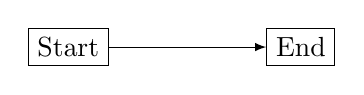
\begin{tikzpicture}
              \node[draw] (start) { Start };
              \node[draw, right=2cm of start] (end) { End };
              \draw[-latex] (start) -- (end);
            \end{tikzpicture}
            \end{document}
          \end{latexcode*}
    \item The standalone file can be compiled directly or included in the document.
          \begin{latexcode*}{fontsize=\scriptsize}
            % need to pass additional `-shell-escape` argument to the compiler
            \usepackage[mode=buildnew]{standalone}

            \begin{figure}[t]
              \centering
              \includestandalone[width=0.8\linewidth]{./figure} % without the `.tex` extension
              \caption{TikZ Figure in Article}
            \end{figure}
          \end{latexcode*}
  \end{itemize}
\end{frame}

\begin{frame}[fragile]{Formatting Tables}
  \begin{itemize}
    \item The \emph{tabular} environment defines the table
    \item Use package \href{http://texdoc.net/texmf-dist/doc/latex/booktabs/booktabs.pdf}{\emph{booktabs}} to create professional table
          % \begin{noindent}
          \begin{latexexample}
              \centering\small
              \begin{tabular}{llr}
                \toprule
                \multicolumn{2}{c}{Item} &           \\
                \cmidrule(r){1-2}
                Animal    & Description & Price (\$) \\
                \midrule
                Gnat      & per gram    & 13.65      \\
                          & each        & 0.01       \\
                Gnu       & stuffed     & 92.50      \\
                Emu       & stuffed     & 33.33      \\
                Armadillo & frozen      & 8.99       \\
                \bottomrule
              \end{tabular}
          \end{latexexample}
          % \end{noindent}
    \item More guidance: \url{https://en.wikibooks.org/wiki/LaTeX/Tables}
    \item \href{https://ctan.org/pkg/excel2latex}{\emph{excel2latex}} can be used to generate \LaTeX~code from excel table
  \end{itemize}
\end{frame}

\begin{frame}[fragile]{Subfloats}
  \begin{itemize}
    \item Use package \href{http://texdoc.net/texmf-dist/doc/latex/caption/subcaption.pdf}{\emph{subcaption}} to create subfigures or subtables
          \begin{latexcode}
            \begin{figure}
              \centering
              \begin{subfigure}[b]{0.5\textwidth}
                \includegraphics[width=\textwidth]{gull}
                \caption{A gull}
              \end{subfigure}
              ~%add desired spacing between images, e.g. ~, \quad, \hfill, \\ etc.
              \begin{subfigure}[b]{0.5\textwidth}
                \includegraphics[width=\textwidth]{tiger}
                \caption{A tiger}
              \end{subfigure}
              \caption{Pictures of animals}
            \end{figure}
          \end{latexcode}
  \end{itemize}
\end{frame}

\begin{frame}[fragile]{References}
  \begin{itemize}
    \item You can use \latexinline|\label{<label name>}| to make a label
          \begin{latexcode*}{fontsize=\scriptsize}
            \section{Section Title}\label{sec:label-a}
            \begin{figure}
              ...
              \caption{figure caption}\label{fig:label-b}
            \end{figure}
            \begin{equation}
              E=mc^2 \label{eqn:lable-c}
            \end{equation}
          \end{latexcode*}
    \item Use \latexinline|\ref{<label name>}| to reference them
    \item Use package \href{http://texdoc.net/texmf-dist/doc/latex/hyperref/manual.pdf}{\emph{hyperref}} to generate pdf hyperlink and create url e.g.~\latexinline|\url{https://google.com}|
    \item Use package \href{http://texdoc.net/texmf-dist/doc/latex/cleveref/cleveref.pdf}{\emph{cleveref}} for auto infer reference types  \\
          e.g.~\latexinline|\cref{fig:label}| is equivalence to \latexinline|Fig.~\ref{fig:label}|
    \item Use \latexinline|\footnote{...}| to insert footnote
  \end{itemize}
\end{frame}

\begin{frame}[fragile]{Theorems}
  \begin{itemize}
    \item There are many packages to offer theorem environments.
    \item Here, we use \latexinline|\usepackage{amsthm,thmtools}|
    \item Declare the theorem environments (document \texdoc{thmtools}{http://texdoc.net/texmf-dist/doc/latex/thmtools/thmtools.pdf})
          \begin{latexcode*}{fontsize=\scriptsize}
            \declaretheorem[style=plain]{axiom}
            \declaretheorem[style=definition]{definition}
            \declaretheorem[style=definition]{example}
            \declaretheorem[style=plain]{lemma}
            \declaretheorem[style=plain]{theorem}
            \declaretheorem[style=remark]{remark}
          \end{latexcode*}
    \item Use it in the document
          \begin{latexcode*}{fontsize=\scriptsize}
            \begin{theorem}[Euclid]
              For every prime $p$, there is a prime $p’>p$.
              In particular, there are infinitely many primes.
            \end{theorem}
          \end{latexcode*}
    \item \latexinline|\usepackage{thm-restate}| to repeat the same theorem multiple times
  \end{itemize}
\end{frame}

\begin{frame}[fragile]{Algorithms}
  \begin{itemize}
    \item There are two common packages to typeset algorithm:
          \begin{itemize}
            \item \href{http://texdoc.net/texmf-dist/doc/latex/algorithm2e/algorithm2e.pdf}{\emph{algorithm2e}}
            \item \href{http://texdoc.net/texmf-dist/doc/latex/algorithmicx/algorithmicx.pdf}{\emph{algorithmicx}}
          \end{itemize}
    \item Example using algorithm2e:
          \begin{latexexample}
            \begin{algorithm}[H]
              \caption{How to write algorithms}
              \KwData{this text}
              \KwResult{learn to write algorithm}
              initialization\;
              \While{not at end of this document}{
                read current\;
                \eIf{understand}{
                  go to next section\;
                  current section becomes this one\;
                }{
                  go back to the beginning\;
                }
              }
            \end{algorithm}
          \end{latexexample}
  \end{itemize}
\end{frame}

\begin{frame}[fragile]{Source Code Highlight}
  \begin{itemize}
    \item Using package \href{http://texdoc.net/texmf-dist/doc/latex/listings/listings.pdf}{\emph{listings}} to highlight the source code.
          % \begin{noindent}
        \begin{latexexample}
    \begin{lstlisting}[language=Python]
    def fib():
      a, b = 0, 1
      while 1:
        yield a
        a, b = b, a + b
    \end{lstlisting}
        \end{latexexample}
        % \end{noindent}
    \item Alternatively, use \latexinline|\lstinputlisting[opt]{file path}| to read code from another file.
    \item Package \href{http://texdoc.net/texmf-dist/doc/latex/minted/minted.pdf}{\emph{minted}} offers more features and better highlights. But it requires:
          \begin{itemize}
            \item Install Pygments \url{http://pygments.org}
            \item Pass additional argument \bashinline|-shell-escape| to the compiler
          \end{itemize}
  \end{itemize}
\end{frame}

\begin{frame}[fragile]{Bibliography}
  \begin{itemize}
    \item \mintinline{text}|.bib| file acts as a database of references, and only includes in the bibliography those references you cite in your paper
          \begin{center}
            \begin{minipage}{0.45\linewidth}
              \inputminted[fontsize=\scriptsize]{bibtex}{./minted/article.bib}
            \end{minipage}\quad%
            \begin{minipage}{0.5\linewidth}
              \inputminted[fontsize=\scriptsize]{bibtex}{./minted/inproceedings.bib}
            \end{minipage}
          \end{center}
    \item More examples can be found in
          \begin{itemize}
            \item \url{http://web.mit.edu/rsi/www/pdfs/bibtex-format.pdf}
            \item \url{https://www.verbosus.com/bibtex-style-examples.html}
          \end{itemize}
  \end{itemize}
\end{frame}

\begin{frame}[fragile]{Bibliography}
  \begin{itemize}
    \item Use \latexinline|\cite{nameofentry}| to cite the referenced paper in the main text
    \item There are two solutions to typeset bibliography
          \begin{itemize}
            \item \textbf{BibTeX}: old and widely support
                  \begin{latexcode}
                    cite some paper~\cite{paperentry}.
                    \bibliographystyle{IEEEtrans}
                    \bibliography{path to bib file}
                  \end{latexcode}
            \item \textbf{BibLaTeX}: new and have more features, document: \texdoc{biblatex}{http://texdoc.net/texmf-dist/doc/latex/biblatex/biblatex.pdfc}
                  \begin{latexcode}
                    \usepackage[style=ieee,giveninits=true,doi=false]{biblatex}
                    \addbibresource{path to bib file}
                    \begin{document}
                    cite some paper~\cite{paperentry}.
                    \printbibliography
                    \end{document}
                  \end{latexcode}
          \end{itemize}
  \end{itemize}
\end{frame}

\section{Advanced Usages}

\begin{frame}[fragile]{More Packages}
  \begin{itemize}
    \item \textbf{Color}: \href{http://texdoc.net/texmf-dist/doc/latex/graphics/color.pdf}{\emph{color}}, \href{http://texdoc.net/texmf-dist/doc/latex/xcolor/xcolor.pdf}{\emph{xcolor}}
          \begin{latexcode}
            \usepackage{color}
            \usepackage[table,dvipsnames]{xcolor}
          \end{latexcode}
    \item \textbf{Draw Boxes}: \href{http://texdoc.net/texmf-dist/doc/latex/tcolorbox/tcolorbox.pdf}{\emph{tcolorbox}}
    \item \textbf{Draw Graphics}: \href{http://texdoc.net/texmf-dist/doc/generic/pgf/pgfmanual.pdf}{\emph{tikz}}, \href{http://texdoc.net/texmf-dist/doc/latex/overpic/overpic.pdf}{\emph{overpic}}
    \item \textbf{Slides}: \href{http://texdoc.net/texmf-dist/doc/latex/beamer/beameruserguide.pdf}{\emph{beamer}}
    \item \textbf{Poster}: \href{http://texdoc.net/texmf-dist/doc/latex/tikzposter/tikzposter.pdf}{\emph{tikzposter}}
    \item \textbf{Miscellaneous}: \href{http://texdoc.net/texmf-dist/doc/latex/microtype/microtype.pdf}{\emph{microtype}}, \href{http://texdoc.net/texmf-dist/doc/latex/footmisc/footmisc.pdf}{\emph{footmisc}}, \href{http://texdoc.net/texmf-dist/doc/latex/preprint/balance.pdf}{\emph{balance}}
  \end{itemize}
\end{frame}

% \begin{noindent}
\begin{frame}[fragile]{Define Commands and Environment}
  \begin{itemize}
    \item Define command using: \latexinline|\newcommand{\name}[num]{definition}|
          \begin{latexexample}
            \newcommand{\highlight}[1]{%
              {\color{red} #1}%
            }
            \highlight{Text in red}
          \end{latexexample}
    \item Define the command using: \latexinline|\newenvironment{name}[num]{before}{after}|
          \begin{latexexample}
            \newenvironment{response}{%
              \begingroup
              \textbf{Response}: \itshape
            }{%
              \endgroup
            }
            \begin{response}
              Some response.
            \end{response}
          \end{latexexample}
      \item More information: \url{https://en.wikibooks.org/wiki/LaTeX/Macros}
  \end{itemize}
\end{frame}
% \end{noindent}

\begin{frame}[fragile]{\LaTeX~Engines}
  \begin{itemize}
    \item There are several \LaTeX~engines
          \begin{itemize}
            \item \alert{pdflatex}: most commonly used
            \item \alert{xelatex} and \alert{lualatex}: new, offer more features
                  \begin{itemize}
                    \item better font support, typeset other language than English, etc
                  \end{itemize}
          \end{itemize}
    \item To compile \LaTeX~manually, you usually need run multiple commands
          \begin{bashcode*}{fontsize=\scriptsize}
            pdflatex root_file
            bibtex root_file # or `biber root_file` if using biblatex
            pdflatex root_file
            pdflatex root_file
          \end{bashcode*}
    \item Or use \bashinline|latexmk| to automatically run commands for you
          \begin{bashcode*}{fontsize=\scriptsize}
            latexmk -pdf root_file # use pdflatex
            latexmk -xelatex root_file # use xelatex
            latexmk -lualatex root_file # use lualatex
          \end{bashcode*}
    \item Some \LaTeX~editors (such as VSCode with LaTeX Workshop, Vim with vimtex) use \bashinline|latexmk| under the hook
  \end{itemize}
\end{frame}

\begin{frame}[fragile]{Other Common Line Tools}
  \begin{itemize}
    \item \textbf{latexmk}
          \begin{itemize}
            \item In addition to build project, it can also be used to clean up auxiliary files
                  \begin{bashcode*}{fontsize=\scriptsize}
                    latexmk -c
                  \end{bashcode*}
            \item It is highly customizable. You can create \mintinline{bash}|.latexmkrc| file to configure \bashinline|latexmk|. \\ document: \texdoc{latexmk}{http://texdoc.net/texmf-dist/doc/support/latexmk/latexmk.pdf}
                  \inputminted[fontsize=\scriptsize]{perl}{./minted/latexmkrc}
          \end{itemize}
    \item \textbf{chktex}: Lint the \LaTeX{} source code for common problem. document: \texdoc{chktex}{http://texdoc.net/texmf-dist/doc/chktex/ChkTeX.pdf}
    \item \textbf{latexindent}: Format the \LaTeX{} source code. document: \texdoc{latexindent}{http://texdoc.net/texmf-dist/doc/support/latexindent/latexindent.pdf}
    \item \textbf{latexdiff}: Marking up difference between \LaTeX{} files. document: \texdoc{latexdiff}{http://texdoc.net/texmf-dist/doc/support/latexdiff/doc/latexdiff-man.pdf}
  \end{itemize}
\end{frame}

\begin{frame}{Further Readings}
  \begin{itemize}
    \item \LaTeX~Wikibooks: \url{https://en.wikibooks.org/wiki/LaTeX}
    \item The Not So Short Introduction to \LaTeXe: \texdoc{lshort}{http://texdoc.net/texmf-dist/doc/latex/lshort-english/lshort.pdf}
    \item Short Math Guide for \LaTeX: \texdoc{short-math-guide}{http://texdoc.net/texmf-dist/doc/latex/short-math-guide/short-math-guide.pdf}
    \item The TeX FAQ List: \url{https://texfaq.org}
    \item LaTeX Stack Exchange: \url{https://tex.stackexchange.com}
    \item Always remember to use \alert{Google} when you encounter problems
  \end{itemize}
\end{frame}

\begin{frame}[standout]
  Thanks \\
  Questions?
\end{frame}

\end{document}
